% Section content template for individual Educative lessons
% This file contains the actual content for a specific section
% Generated from Educative API section content

% Section: AI Evaluation of Building Blocks in Online Education System
% Section ID: 6068850835718144
% Section Slug: ai-evaluation-of-building-blocks-in-online-education-system
% Generated: 2025-12-07T22:22:13.700624

\subsection{Online education system}\label{Online-education-platform}
\\
The following is a high-level system design of an online education system that provides different types of video tutorials for various subjects. Users opt for courses to buy and watch video tutorials. Take a look at the architecture to answer the questions provided below. The details of different types of services included in the design are also given.

In the system, each service is described below:

\begin{itemize}
\tightlist
\item
\textbf{Application servers:} The application servers receive user requests and forward them to the relevant services. Their main purpose is to host, manage, and execute applications, execute user requests, and manage connections with databases and other services.
\item
\textbf{Search service:} This service helps users to find relevant courses on the platform.
\item
\textbf{Shopping cart service:} This service is responsible for keeping the courses that are selected by the users for purchase.
\item
\textbf{Order management service:} This service is responsible for the entire process, from order placement to order fulfillment. It includes tasks like validating orders, processing payments, handling returns and refunds, and offering customer support.
\item
\textbf{Recommendation service:} This service provides personalized content recommendations to users based on their preferences, behavior, and learning goals.
\item
\textbf{Video processing service:} This service handles the tasks of video transcoding, uploading, and on-demand streaming for video tutorials. Its primary users are the administrators who rely on it to upload educational videos.
\item
\textbf{Content delivery network (CDN):} The CDN distributes web content consisting of HTML pages, JavaScript files, images, videos, and other media files to users in various geographic locations.
\item
\textbf{Pub-sub service:} The pub-sub service decouples different services and enables asynchronous communication between them.
\end{itemize}

\begin{figure}[htbp]
 \centering
 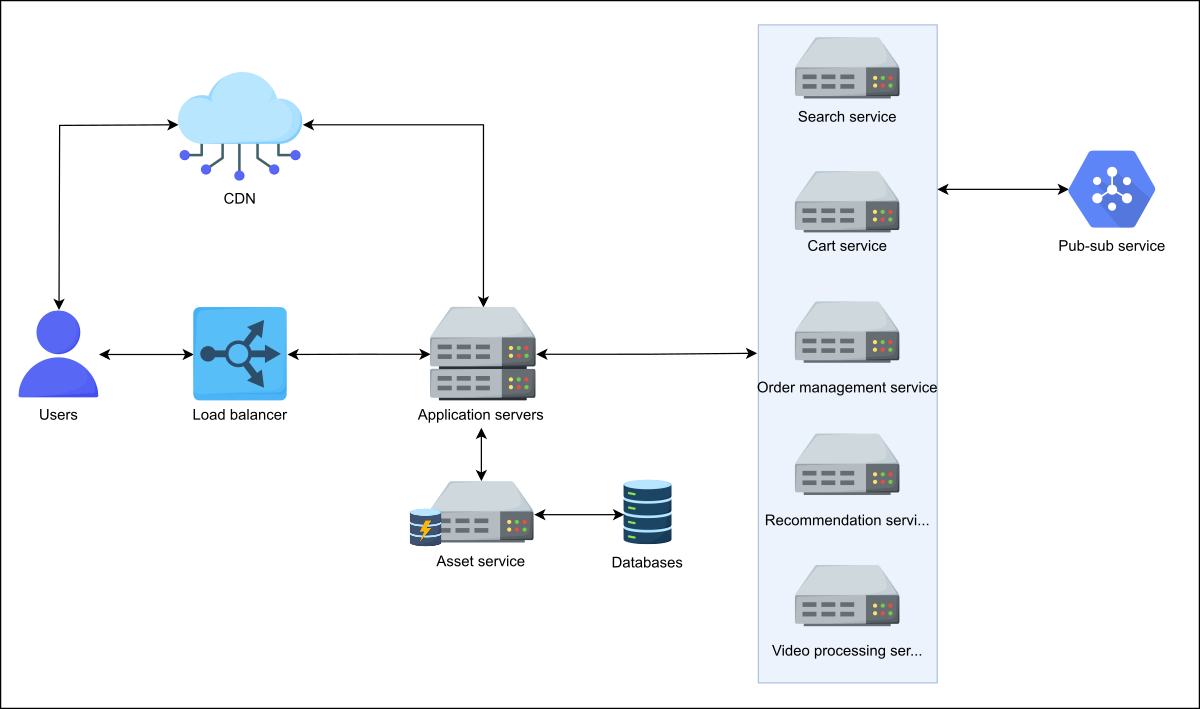
\includegraphics[width=0.5\textwidth]{Images/chapter_25/section_6068850835718144/5793704323710976.png}
 \caption{An abstract system design of an online education system}
\end{figure}

As we can see, the given design is simplified, but there are certain issues that the system faces, which we've listed below. In this exercise, your task is to identify the building blocks that, if incorporated, can remove these problems for optimal operation of the system. Here are the problems the system is currently facing:

\begin{enumerate}
\item
If certain users continuously send an excessive number of requests (probably a denial of service attack), the system could potentially overwhelm our back-end servers. It 's imperative to mitigate such request surges to prevent any adverse impact on the server infrastructure. Which component do you think can help fix this issue?
\item
Suppose we're managing a user base of 200 million, and they're generating a massive volume of requests across various categories, for example, video uploads, comments, forum discussions, and module additions. Managing and distinguishing these activities within the system can be a challenge. To efficiently address this issue and uniquely identify each request, which component or building block is needed?
\item
The engineering team currently invests a significant amount of time in identifying and troubleshooting system failures. To streamline this process, it's crucial to integrate an appropriate building block or service into the system design. What component do you recommend for identifying and troubleshooting failures in the system?
\item
Besides the drawbacks, we want to add a feature to allow users to see the number of views on each video tutorial. Essentially , we need a counter to keep a count of the large number of views on a video. What approach would you propose to efficiently estimate the approximate number of views in this high-traffic environment?
\end{enumerate}
\\
\textbf{Note:} Please provide answers in the same order as that of the questions.

\textbf{Question:}

Improve the system design of an online education system.

\textbf{Reference Answer:}

The answers to the above questions are given below in the same sequence as that of the \#Questions:

\begin{enumerate}
\def\labelenumi{\arabic{enumi}.}
\tightlist
\item
To manage and mitigate the impact on backend servers due to a vast number of incoming requests, we should incorporate a rate limiter with a suitable rate-limiting algorithm.
\item
To assign unique identifiers to different requests and events occurring within the system, we should incorporate the sequencer building block in the system.
\item
The system should encompass a monitoring service to reduce the time required for problem identification and troubleshooting.
\item
To efficiently estimate the number of views in high-traffic environments, we need a building block known as a sharded counter.
\end{enumerate}

% End of section content